% Chapter 1

\chapter{Introducción} % Main chapter title

\label{Chapter1} % For referencing the chapter elsewhere, use \ref{Chapter1} 

%----------------------------------------------------------------------------------------

% Define some commands to keep the formatting separated from the content 
\newcommand{\keyword}[1]{\textbf{#1}}
\newcommand{\tabhead}[1]{\textbf{#1}}
\newcommand{\code}[1]{\texttt{#1}}
\newcommand{\file}[1]{\texttt{\bfseries#1}}
\newcommand{\option}[1]{\texttt{\itshape#1}}

%----------------------------------------------------------------------------------------

\section{Tema principal}

\ttitle.


%----------------------------------------------------------------------------------------

\section{Objetivo General}

Aplicar conceptos del estado del arte a un problema que ha recibido poca atención en el área de procesamiento de lenguaje natural (NLP, por sus siglas en inglés). Esto con el propósito de demostrar la capacidad de las redes neuronales recurrentes (RNN) y \emph{transfer learning} en la tarea específica.

\subsection{Objetivos específicos}

\begin{itemize}
\item Ser pionero en la aplicación de \emph{transfer learning} en la tarea específica de perfilamiento de autores en el área de procesamiento de lenguaje natural.
\item Exponer las ventajas y desventajas de utilizar esta tecnología en esta subtarea.
\item Exponer como caso de uso la utilidad de esta aplicación en distintas áreas, como en el mercadeo.
\item Contribuir a la academia en este campo con los resultados obtenidos
\end{itemize}

%----------------------------------------------------------------------------------------

\section{Introducción}

El campo de \emph{Machine Learning} (aprendizaje de máquinas) y \emph{Deep Learning} (aprendizaje profundo), no son para nada nuevos, pero han sido una gran sensación en los últimos años, cada vez ganando más popularidad. Los primeros conceptos desarrollados en el campo tienen décadas. La primer red neuronal --- la base del modelo a utilizar en este trabajo y la base del aprendizaje profundo --- fue planteada en los años 90. ¿Qué, entonces, ha cambiado en los últimos años que ha generado una explosión en el campo? La disponibilidad de los datos. Con el surgimiento y la penetración cada vez más alta del internet se han abierto las puertas a una cantidad de datos nunca antes vista.

La revolución de los datos ha llevado a la comunidad científica y a las industrias a recolectar grandes cantidades de datos e información y organizarlos de forma que se puedan interpretan y se pueda obtener valor de la misma.

Los sistemas de aprendizaje profundo necesitan pasar por una fase de aprendizaje (comunmente llamada fase de entrenamiento) y estos modelos tienen la característica de necesitar cantidades masivas de datos para poder generalizar bien lo aprendido en su fase de entrenamiento. Esto combinado con la explosión de datos ha llevado a que el campo tenga un surgimiento en todas las áreas de software, mostrando mucha promesa en algunos campos en específico como \emph{Computer Vision} (visión de computadoras, CV) y en NLP.

Conforme ha avanzado el campo se ha determinado que para algunas tareas en específico no se cuenta con la cantidad necesaria para poder obtener un modelo competente. Esto ha llevado al desarrollo de una técnica llamada \emph{Transfer Learning} que permite utilizar un modelo pre-entrenado en una tarea más general que la deseada y poder realizar ajustes específicos para una tareá más acotada. Este proceso de ajuste requiere de una cantidad de datos considerablemente menor a entrenar un modelo completamente desde cero.

La técnica de \emph{transfer learning} ha permitido muchos avances en el área de CV específicamente. Este trabajo intenta mostrar la habilidad que se tiene de aplicar este concepto en un área distinta como NLP, específicamente en la tarea de perfilamiento de autores.

\section{Planteamiento del problema}

En el área de NLP han existido técnicas poderosas por décadas que abusan de algunas suposiciones que no siempre son ciertas y se basan en simples métodos estadísticos que asignan valores a características del texto. El campo también ha dependido de ingeniería de características en los datos, lo cual significa que hay esfuerzos activos serios en analizar cada sub-tarea a fondo y determinar cuáles serían los mejores determinantes de un resultado deseado, p.e. las carecterísticas principales que determinan la categoría que se le debe asignar un texto.

\begin{figure}
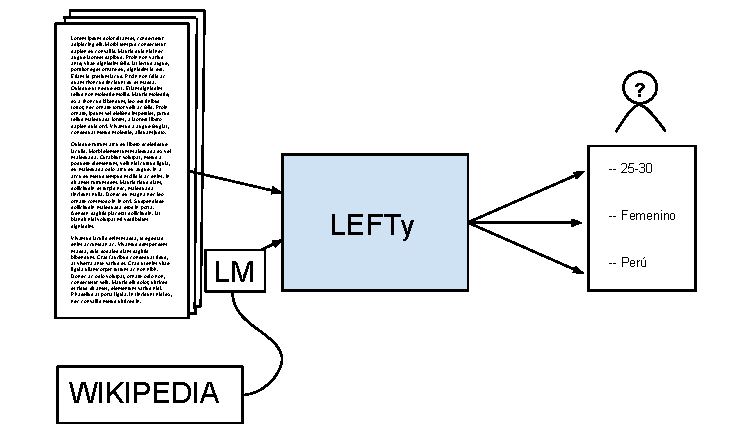
\includegraphics[scale=1.0]{Figures/projectstruct.pdf}
\caption{Estructura del proyecto planteado en este trabajo de investigación. La figura está diseñada para propósitos ilustrativos. \textit{LM} denota el modelo de lenguaje el cual es preentrenado con texto de wikipedia, lo cual es un paso previo.}
\label{fig:projstruct}
\end{figure}

En áreas como mercadeo y ciencias forenses hay una necesidad de identificar textos escritos por autores desconocidos, obtener características de los mismos y poder categorizarlos de forma no manual. Esto con el fin de poder, en el caso de mercadeo, orientar mejor la publicidad de ciertos productos a una audiencia apropriada. En el área forense con el fin de identificar a sospechosos vinculados a algún crimen a partir de un texto anónimo obtenido en el contexto del caso.

Habiendo planteado lo anterior, la necesidad de un sistema automatizado sea capaz de no sólo extraer información de un texto anónimo de forma precisa y confiable, sino de también hacerlo sin necesidad de hacer una ingeniería de características claves para cada posible parámetro que se quiera obtener de los textos.

De esto sigue que los requisitos para este proyecto sean los siguientes:

\begin{itemize}
\item Permitir elegir datos a obtener de un texto anónimo (siempre y cuando se tenga la información disponible).
\item Realizar el entrenamiento para obtener los datos de forma rápida y con demandas de hardware modestas.
\item Una vez el entrenamiento esté completo, permitir realizar predicciones sobre textos anónimos con los datos a obtener elegidos.
\item Permitir la automatización de predicciones ofreciendo un servicio web fácil de consultar.
\end{itemize}

La figura \ref{fig:projstruct} muestra la estructura del proyecto planteado, el cual llenaría los requisitos expuestos en esta sección de forma ilustrativa. El flujo de la información tendría esa forma y las predicciones mostradas son ejemplos de posibilidades.

\section{Resumen}

El proyecto deberá tener la flexibilidad de poder adaptarse a las necesidades del caso de uso espcífico que se le dé y a la vez tener la capacidad predictiva de un modelo del estado del arte. El modelo utilizará tecnologías de aprendizaje profundo por ser la tecnología más prometedora en este campo.





